\documentclass{article}
\usepackage[utf8]{inputenc}
\usepackage[T1]{fontenc}
\usepackage[frenchb]{babel}
\usepackage[bookmarks=true]{hyperref}
\usepackage{lmodern}
\usepackage{graphicx}


\author{Gentile Pierre, Didier-Roche François}
\date{\today}
\title{Document de conception générale}

\frenchbsetup{StandardLists=true}

\begin{document}

\maketitle

\newpage
\tableofcontents
\newpage


\section{Introduction}
\subsection{Objet}


\subsection{Portée du document}

\subsection{Définitions, acronymes, abréviations}

\subsection{Références}

\subsection{Vue d'ensemble}
Dans la suite du document, nous verrons dans un premier temps quels sont les acteurs et comment peuvent t'ils agir sur le système. Nous verrons ensuite via des diagrammes


\section{Cas d'utilisation}
\subsection{Acteurs}
\subsubsection{Utilisateur dit "particulier"}
Un utilisateur dit "particulier" est un utilisateur recherchant un service proposé par un utilisateur dit "profesionnel".
Ces utilisateurs constituent la majorité des usagers de l'application.
Il n'auront pas la possibilité de
\begin{itemize}
  \item proposer des services.
  \item d'avoir un calendier de rendez-vous.
  \item d'avoir une entrteprise.
\end{itemize}
Ils auront la possibilité de
\begin{itemize}
  \item rechercher des services et/ou des professionnels.
  \item prendre un rendez-vous pour un service.
  \item de payer directement via l'application certains professionnels.
  \item d'acceder à la gestion de son compte.
\end{itemize}


\subsubsection{Utilisateur dit "professionnel"}
Un utilisateur dit "professionnel" est un utilisateur proposant un ou plusieurs service(s) aux utilisateurs dit "profesionnel".
Ces utilisateurs constituent la minorité des usagers de l'application.
Un utilisateur dit "professionnel" aura la possibilité de
\begin{itemize}
  \item proposer des services.
  \item gerer des services.
  \item d'avoir un calendier de rendez-vous.
  \item gerer son calendrier de rendez vous.
  \item d'avoir une entrteprise.
  \item gerer son entreprise (descripions, horaires).
  \item profiter des mêmes services que les utilisateurs dit "particuliers".
\end{itemize}


\subsection{Liste et diagrammes de cas d'utilisation}
\subsubsection{Inscription}
Ce cas permet de s'inscrire sur l'application en tant que particulier ou professionnel.
Dans le cas d'un professionnel, ce dernier pourra ensuite profiter des droits qui lui sont accordés.

\begin{center}
  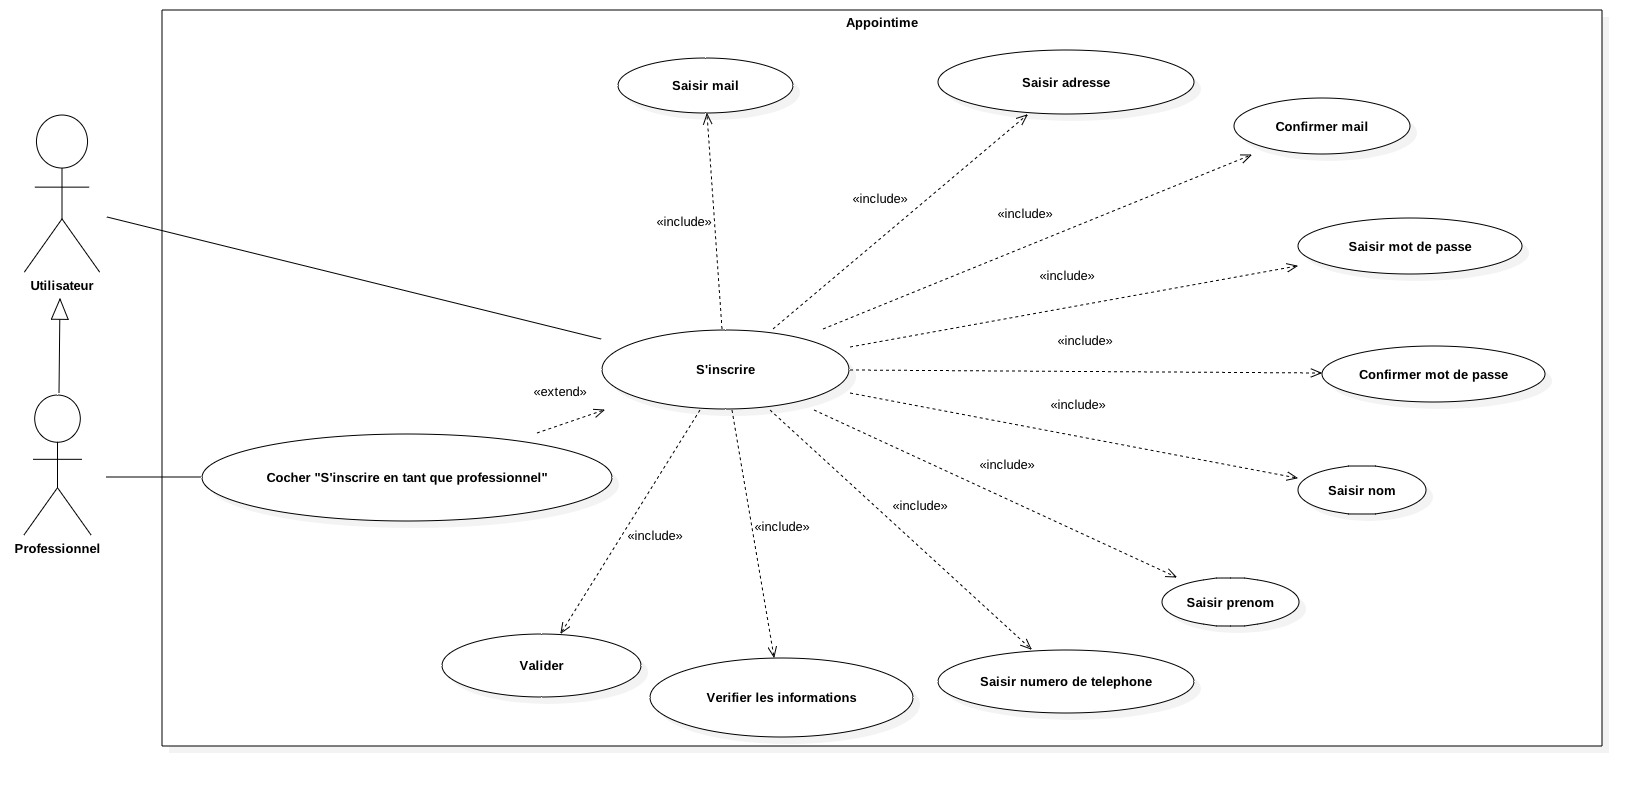
\includegraphics[width=400pt]{diagram/useCaseInsc}
\end{center}


\subsubsection{Gestion de compte}
Ce cas permet de modifier ses informations
\begin{center}
  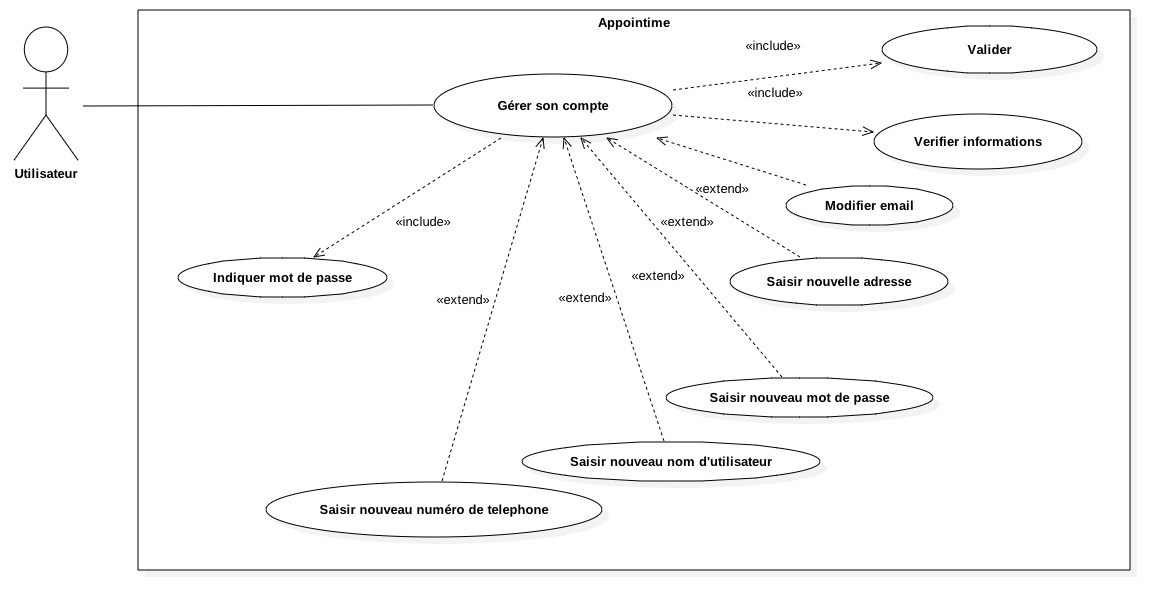
\includegraphics[width=400pt]{diagram/useCaseGererCompte}
\end{center}

\subsubsection{Connexion}
Ce cas permet de se connecter à l'application.
\begin{center}
  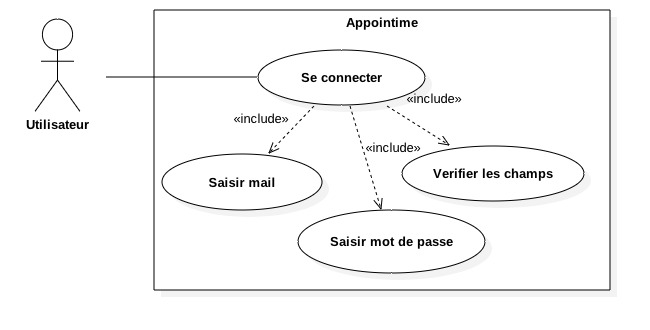
\includegraphics[width=400pt]{diagram/useCaseConnexion}
\end{center}

\subsubsection{Création d'une entreprise}
Ce cas permet à un professionnel de créer son entreprise et de renseigner les informations relatives a celle ci apres son inscription.
\begin{center}
  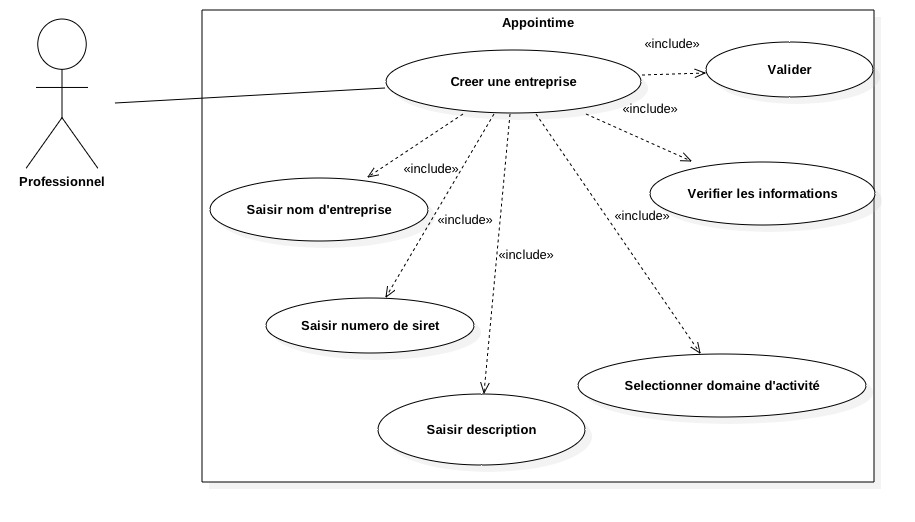
\includegraphics[width=400pt]{diagram/useCaseCreerEntreprise}
\end{center}


\subsubsection{Recherche de professionnel}
Ce cas permet à un utilisateur de rechercher un professionnel via un nom, un secteur d'activité ou un flashcode.
\begin{center}
  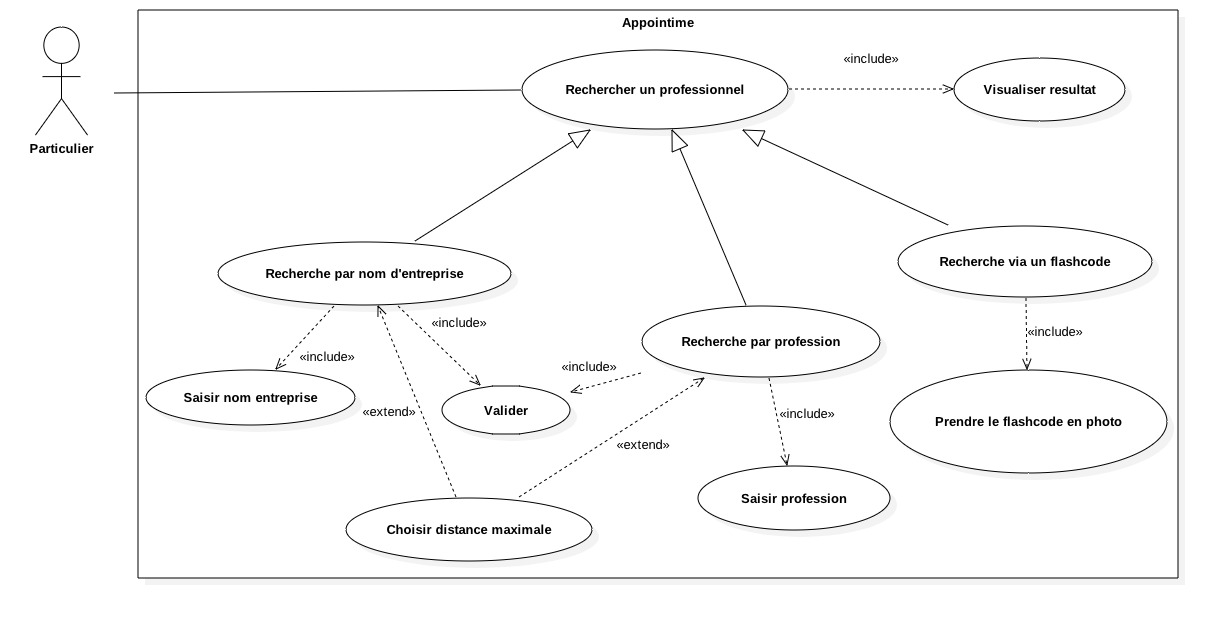
\includegraphics[width=400pt]{diagram/useCaseRecherchePro}
\end{center}

\subsubsection{Gestion des horaires}
Ce cas permet à un professionnel de gérer les horaires d'ouverture de son entreprise.
\begin{center}
  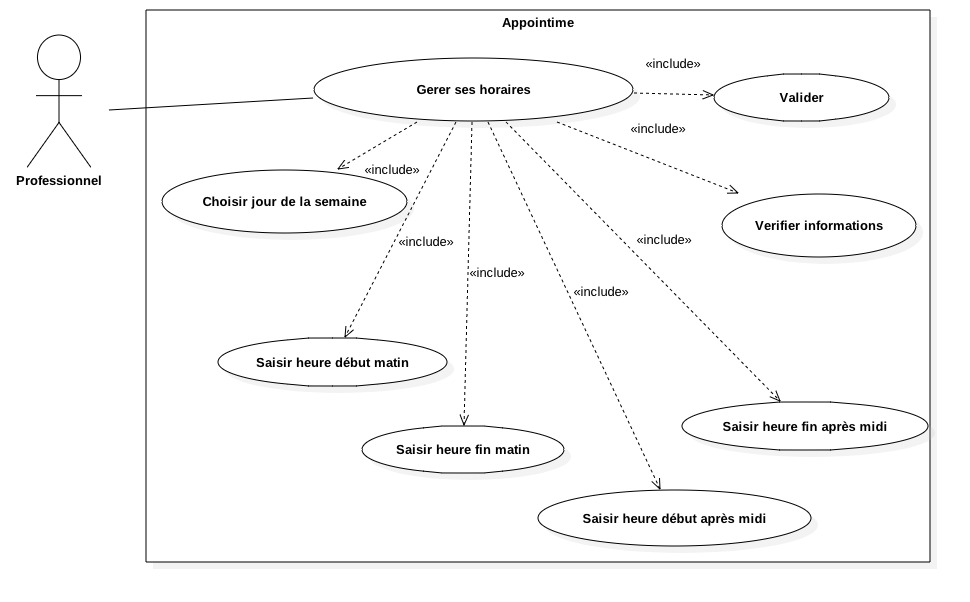
\includegraphics[width=400pt]{diagram/useCaseGererHoraire}
\end{center}

\subsubsection{Création de préstation}
Ce cas permet à un professionnel de créer une prestation
\begin{center}
  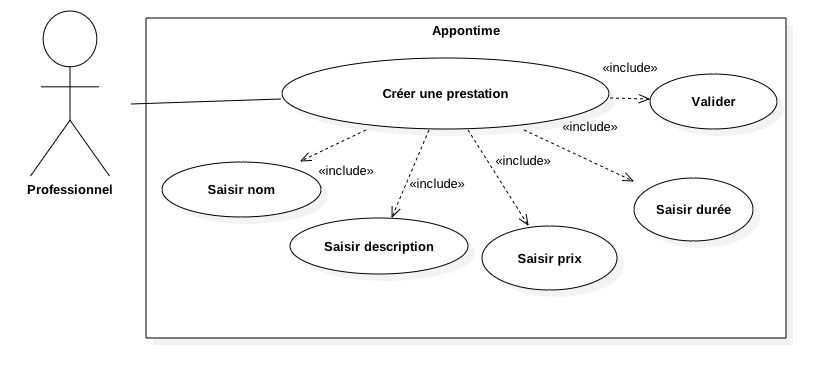
\includegraphics[width=400pt]{diagram/useCaseCreerPrestation}
\end{center}
\subsubsection{Prise de rendez-vous}
Ce cas permet de prendre un rendez vous chez un professionnel à une horaire libre.
\begin{center}
  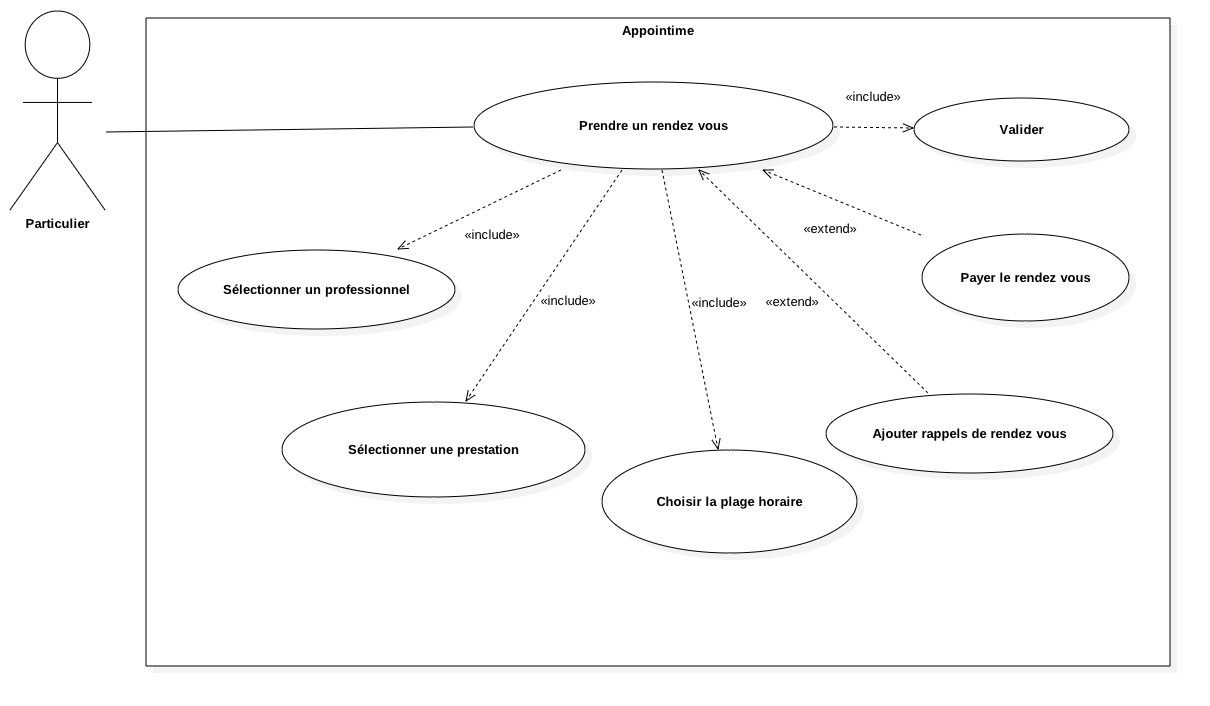
\includegraphics[width=400pt]{diagram/useCasePriseRdv}
\end{center}
\subsubsection{Confirmation de rendez vous}
Ce cas permet a un professionnel de confirmer ou non un rendez vous pris préalablement par un particulier.
\begin{center}
  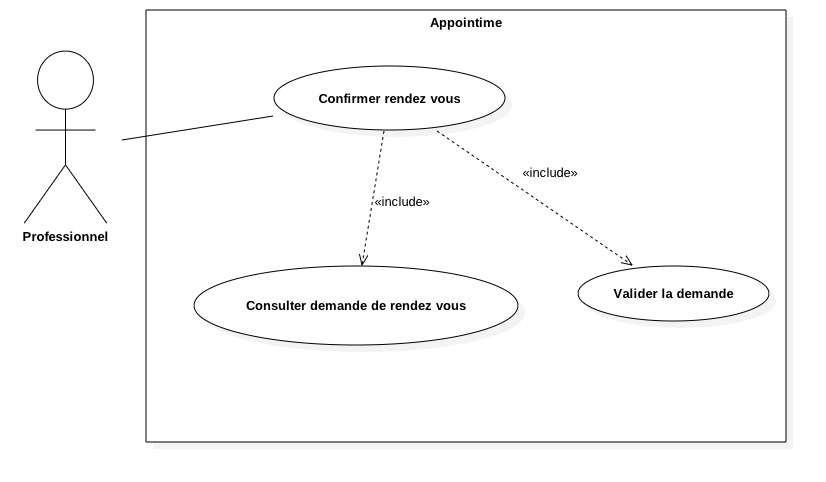
\includegraphics[width=400pt]{diagram/useCaseConfirmerDemande}
\end{center}
\section{Diagrammes d'activité}
\subsection{Inscription}
\begin{center}
  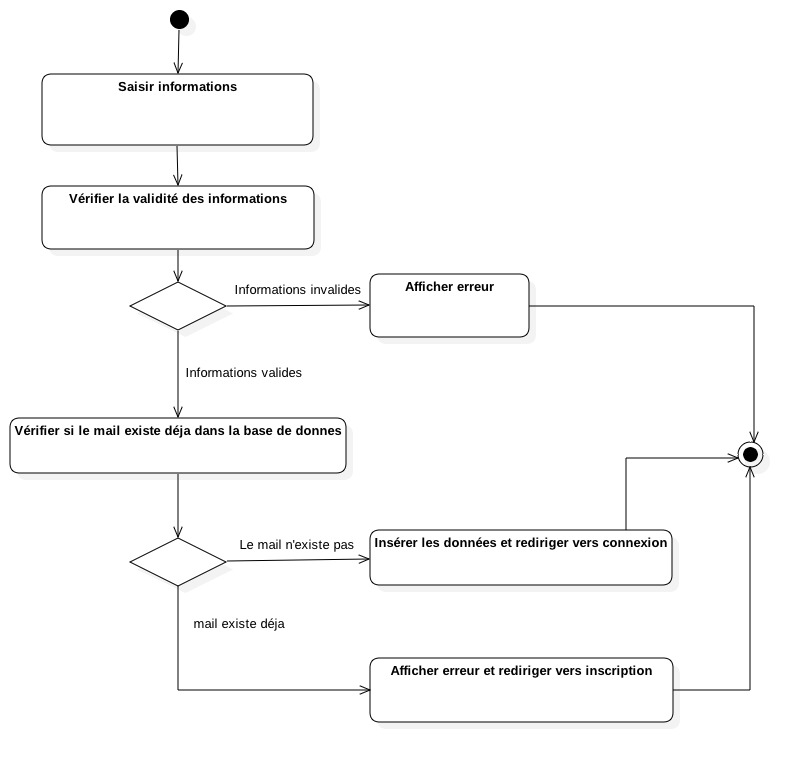
\includegraphics[width=400pt]{diagram/activiteInscription}
\end{center}
\subsection{Connexion}
\begin{center}
  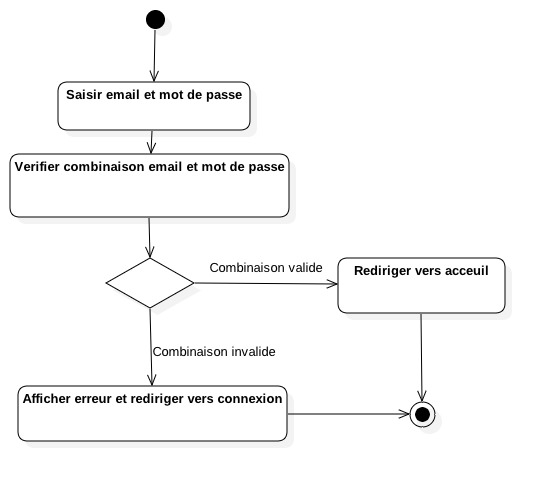
\includegraphics[width=400pt]{diagram/activiteConnexion}
\end{center}
\subsection{Création d'une entreprise}

\subsection{Création de préstation}

\subsection{Prise de rendez-vous}

\section{Diagrammes de séquence}
insc+conn+recherche+priserdv particuliers
creationPrestation pro

\section{Description et interaction des classes}
\subsection{Description des classes}

\subsection{Diagramme de classe}

\section{Description de la persistance des données}
\subsection{Modèle entité association}















\end{document}
